\chapter{Análisis de Resultados}

\par En este capitulo se describirá el simulador desarrollado con sus condiciones de diseño, limitaciones, suposiciones, validaciones, funcionalidades y sus posibles usos y aplicaciones.

\section{Horno simulado}

\par El horno escogido es de tipo cabina de simple fuego, con una capacidad de carga de 23 megavatios, o el equivalente aproximado de un cambio de 50 ºC para un flujo de 16 mil metros cúbicos por día de residuo de petroleo con gravedad especifica de 0.84.

\par Estas variables de diseño pueden ser modificados en un futuro pero se tomaron por los datos disponible para comparar contra la simulación.

\subsection{Diseño mecánico}

\par Se puede observar a detalle cada una de las dimensiones en la Figura \ref{apx:img} ampliada en los anexos, estas dimensiones responden a la distribución interna de los tubos para el fluido y sus configuraciones por sección.

\begin{figure}[hbt]
\begin{center}
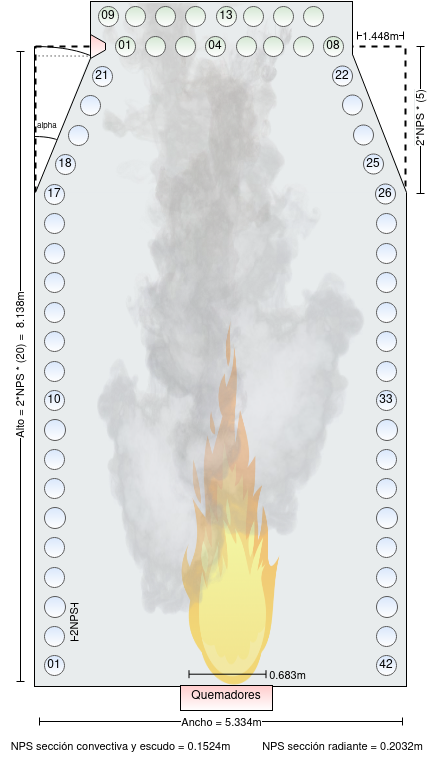
\includegraphics[scale=0.45]{images/firebox}
\caption[Diagrama de la cámara de combustión algoritmo]{Diagrama de la cámara de combustión del horno simulado.}
\label{fig:firebox}
\end{center}
\end{figure}

\par En la tabla \ref{tbl:firebox} se muestran las dimensiones de la cámara de combustión, mostradas en pies para su correspondiente uso en el cálculo de la longitud promedio de láser, y se pueden denotar los detalles del techo de la cámara en la Figura \ref{fig:firebox}.

\begin{table}
\begin{center}
\caption[Dimensiones de la cámara de combustión]{Dimensiones de la cámara de combustión, mostrada en pies para su uso en la ecuación \ref{eq:pl} y la tabla \ref{tbl:mbl}}
\label{tbl:firebox}
\begin{tabular}{c|c}
Altura interna, ft	& 27.407 \\
Largo interno, ft 	& 64.552 \\
Ancho interno, ft 	& 17.500 \\
\end{tabular}
\end{center}
\end{table}

\par La descripción detallada de las característica de los tubos y aletas usadas se puede encontrar en la tabla \ref{tbl:tubes} y una vista en perspectiva de la distribución de los tubos se puede apreciar en la Figura \ref{fig:diagrama-meca}.

\begin{table}
\begin{center}
\caption[Distribución de tubos en el horno]{Distribución de tubos en el horno}
\label{tbl:tubes}
\begin{tabular}{l|c|c|c}
Sección 					& Radiante			& Escudo			& Convectiva \\
\hline
Material de tubos			& \multicolumn{3}{c}{-- A-312 TP321 --} \\
Soporte de tubos    		& Interno			& Externo			& Externo		\\
Arreglo			    		& Paralelo			& Escalonado		& Escalonado	\\
No. de tubos total    		& 42				& 16				& 40			\\
No. de tubos por fila		& 2					& 8					& 8				\\
Grosor pared de tubos, cm	& 0.818				& 0.711				& 0.711			\\
Di. interno de tubos, cm	& 7.981				& 16.827			& 16.827		\\
Espaciado de tubos, cm  	& 40.640			& 					& 				\\
Espaciado transversal, cm  	&					& 30.480			& 30.480		\\
Espaciado longitudinal, cm 	&					& 30.480			& 30.480		\\
Largo de tubos efectivo, m	& 18.926			& 18.288			& 18.288		\\
\hline
Material de aletas			&					& 					& 11.5-13.5Cr	\\
Tipo de aletas				&					& 					& Solidas		\\	
Altura de aletas, cm		&					& 					& 2.438			\\
Grosor de aletas, cm		&					& 					& 0.152			\\
Densidad de aletas, aleta/m	& 					& 					& 196.850		\\
\end{tabular}
\end{center}
\end{table}

\subsection{Combustible seleccionado y aire simulado}

\par Como combustible se utilizó un gas de refinería por ser lo más común en la industria petrolera, la composición molar establecida para hacer las pruebas del algoritmo se describe en la tabla \ref{tbl:combustible}. Sin embargo, la posibilidad de cambiar la composición esta abierta en la interfaz del simulador.

\par El aire ambiental seco establecido para simplificar los cálculos solo contiene \ac{n2} y \ac{o2}, otros compuestos como el \ac{argon} son despreciados por sus aporte del 1\% o menos a las ecuaciones de combustión. Como se describió en la sección de combustión del capitulo 2, la composición tomada para el aire seco es 20.95\% de \ac{o2} y 79.05\% de \ac{n2}.

\par La humedad relativa del aire establecida en las pruebas fue del 50\% con una temperatura ambiente de 26.667 ºC.

\begin{table}
\begin{center}
\caption[Composición del combustible base]{Composición molar porcentual del combustible base.}
\label{tbl:combustible}
\begin{tabular}{l|r}
	Gas combustible					& (Moles \%) \\
	\hline
	Metano ($CH_4$)					& 56.470 \\
	Etano ($C_2H_6$)				& 15.150 \\
	Propano ($C_3H_8$)				& 6.220 \\
	n-Butano ($C_4H_{10}$)			& 1.760 \\
	i-Butano ($C_4H_{10}$)			& 0.750 \\
	Etileno ($C_2H_4$)				& 1.580 \\
	Propileno ($C_3H_6$)			& 2.770 \\
	Monóxido de carbono ($CO$)		& 0.660 \\
	Dióxido de carbono ($CO_2$)		& 2.540 \\
	Hidrógeno ($H_2$)				& 11.420 \\
	Nitrógeno ($N_2$)				& 0.680 \\
	Agua ($H_2O$)					& 0.000 \\
	Oxigeno ($O_2$)					& 0.000 \\
	Sulfuro de hidrógeno ($H_2S$)	& 0.000 \\
\end{tabular}
\end{center}
\end{table}

\subsection{Datos y resultados de la combustión simulada}
\par Luego de correr la simulación desarrollada, en la sección de combustión, se obtuvieron los datos de la tabla \ref{tbl:combustion-data}, adicionalmente, la composición del gas de combustión resultante se describe en la tabla \ref{tbl:combustion-gas}.

\begin{table}
\begin{center}
\caption[Datos de la combustión]{Datos de la combustión simulada.}
\label{tbl:combustion-data}
\begin{tabular}{l|c}
	Exceso de aire, \%								& 20.000 \\
	Humedad relativa, \%							& 50.000 \\
	Temperatura del aire, °C						& 26.667 \\
	A/C másica teórica requerido					& 15.574 \\
	A/C másica húmeda con exceso de aire			& 18.689 \\
	Unidad de gas de combustión por unidad de aire  & 19.689 \\
	Poder Calorífico Neto  (NCV), kJ/kg				& 45,718.6 \\
	Poder Calorífico Bruto (GCV), kJ/kg				& 50,268.0 \\
	Peso Molecular (PM) del combustible, kg/kmol	& 21.149 \\
	PM del gas de combustión, kg/kmol				& 27.911 \\
\end{tabular}
\end{center}
\end{table}

\par Para validar la confiabilidad de estos resultados se compararon con los obtenidos en el software privado de diseño de hornos, WinHeat\copyright, con más de 25 años de trayectoria en el mercado, resultados probados en campo y con una subscripción anual valorada en \$4.000.

\par La conclusión de esta comparación arrojó que la diferencia entre los resultados de ambos simuladores es menor al 0.1\% en esta sección.

\begin{table}
\begin{center}
\caption[Composición del gas de combustión]{Composición molar y másica porcentual del gas de combustión}
\label{tbl:combustion-gas}
\begin{tabular}{l|c|c|c}
		& \% Peso & \% Moles \\
	\hline
	Nitrógeno ($N_2$)			& 72.121	& 71.860 \\
	Oxígeno ($O_2$)				& 3.636 	& 3.172	 \\
	Dióxido de carbono ($CO_2$)	& 13.753	& 8.723	 \\
	Vapor de agua ($H_2O$)		& 10.490	& 16.245 \\
	Dióxido de azufre ($SO_2$)	& 0.000 	& 0.000	 \\
	Monóxido de carbono ($CO$)	& 0.000 	& 0.000	 \\
\end{tabular}
\end{center}
\end{table}

\subsection{Datos de la secciones de transferencia de calor}

\par Datos de comparación se muestran en las tablas \ref{tbl:compara-zr}, \ref{tbl:compara-ze} y \ref{tbl:compara-zc}.

\par En estas tablas se pueden apreciar las diferencias dentro de cada sección del simulador contra los resultados del simulador privado de referencia WinHeat\copyright, en las distribuciones de calor la diferencia máxima es de 2.5\%, esto desencadena diferencias en las temperaturas de entrada y salida internas del gas de combustión y del fluido de proceso, naturalmente al cambiar la distribución del calor por sección esta se refleja en los valores intermedios.

\begin{table}
\begin{center}
\caption[Resultados en zona radiante de intercambio de calor]{Comparación de resultados en zona radiante de intercambio de calor.}
\label{tbl:compara-zr}
\begin{tabular}{l|c|c}
	& Sim EC 2022 & WinHeat\copyright \\
Temperatura entrada fluido, °C	& 379 & 378	\\
Temperatura salida fluido, °C	& 411 & 411	\\
Temperatura pared de tubo, °C	& 432 & 459	\\
Temperatura salida gas, °C	    & 798 & 813	\\

Masa de combustible, kg/s		& 0.574 & 0.564	\\
Calor combustión, MW			& 26.233 & 25.790	\\
Calor aire, MW					& 0.123 & 0.119	\\
Calor combustible, MW			& 0.022 & 0.000	\\

Calor gas de combustión, MW		& 11.083 & 10.615	\\
Calor de perdidas, MW			& 0.393 & 0.226	\\
Calor radiante a escudo, MW		& 1.747 & 1.665	\\
Calor de convección, MW			& 1.705 & 1.650	\\
Calor de radiación, MW			& 11.443 & 11.753	\\
Calor del fluido, MW			& 13.154 & 13.417	\\

Distribución de calor radiante, \%	& 62.78 & 64.01 \\

Área total (At), m$^2$				& 547.09 & 547.01 \\
Área refractaria (Ar), m$^2$		& 566.42 & 541.70 \\
Área de plano frío (Acp), m$^2$		& 323.05 & 369.73 \\
Factor de eficiencia alfa			& 0.904 & 0.904 \\

Coef. de conv. int., kJ/h-m$^2$-C	& 2,770.4 & 2,992.7 \\
Coef. de conv. ext., kJ/h-m$^2$-C	& 30.663 & no reporta \\

Longitud media de láser (MBL), ft	& 20.829 & 20.45 \\
P$_{CO_2}$+P$_{H_2O}$, atm 		    & 0.249 & 0.250 \\
\end{tabular}
\end{center}
\end{table}

\par La temperatura de chimenea, a la cual salen los gases de combustión del horno, es 9 ºC mayor en el simulador desarrollado (2.3\%), lo que repercute en los valores de eficiencia obtenidos.

\par El flujo másico de combustible obtenido es ligeramente mayor (1.77\%) al reporta por el simulador de referencia y la máxima diferencia en las temperaturas internas corresponde a la entrada del gas en la zona convectiva (2.97\%).

\begin{table}
\begin{center}
\caption[Resultados en zona escudo de intercambio de calor]{Comparación de resultados en zona escudo de intercambio de calor.}
\label{tbl:compara-ze}
\begin{tabular}{l|c|c}
	& Sim EC 2022 & WinHeat\copyright \\
Temperatura entrada fluido, °C		& 370 & 369	\\
Temperatura salida fluido, °C		& 379 & 378	\\
Temperatura pared de tubo, °C		& 401 & 407	\\
Temperatura entrada gas, °C			& 798 & 813	\\
Temperatura salida gas, °C			& 694 & 674	\\
Temperatura logarítmica media, K	& 370 & 660 \\
Masa gas de combustión, kg/s	& 11.298 & 11.099	\\

Calor gas de combustión, MW		& 1.593 & no reporta \\
Calor de convección, MW			& 1.592 & 1.957	\\
Calor de radiación, MW			& 1.747 & 1.665	\\
Calor del fluido, MW			& 3.340 & 3.621	\\
Distribución de calor escudo, \%	& 15.89\% &  17.3\% \\

Área total (At), m$^2$				& 154.688 & 158.678 \\
Área de plano frío (Acp), m$^2$		& 44.593 & no reporta \\
Factor de eficiencia alfa			& 1.00 & 1.00 \\

Coef. tran. global (Uo), kJ/h-m$^2$-C	& 100.253  & 121.016 \\
Coef. de conv. int., kJ/h-m$^2$-C	& 4,426.5 & 4,411.3 \\
Coef. de conv. ext., kJ/h-m$^2$-C	& 30.663 & no reporta \\
\end{tabular}
\end{center}
\end{table}

\par Las áreas de transferencia totales de los tubos del horno son iguales en la sección de radiación, 2.5\% menores en la sección de escudo y 4.1\% menores en la sección de convección, donde se incluye en área de las aletas.
\par Por último, con más diferencias observadas, se encuentran los coeficientes de transferencia de calor, en la zona radiante el único reportado por WinHeat\copyright es el coeficiente de convección interno que difiere en 7.1\%, en las otras zonas esta diferencia no supera el 0.5\%; mientras que el coeficiente de transferencia global de la zona de escudo y convección difieren en 17.3\% y 4.2\% respectivamente.
\par Los resultados fueron revisados uno a uno, se tomaron los que mostraron diferencias significativas y fueron corroborados a mano con las ecuaciones disponibles y al comprobar su tendencia en los rangos de diseño del horno, cerrando la aproximación del calor absorbido por el fluido al 0.5\%, se culminó el desarrollo del algoritmo de cálculo con éxito.

\subsubsection{Resultados adicionales}
\par Como resultados adicionales el simulador muestra los valores de emisión de \ac{co2} en toneladas/año, la eficiencia térmica del calor neto (NHV) y calor bruto (GHV)\cite{bib:api560}, con sus respectivos poderes caloríficos asociados.

\begin{table}
\begin{center}
\caption[Resultados en zona convectiva de intercambio de calor]{Comparación de resultados en zona convectiva de intercambio de calor.}
\label{tbl:compara-zc}
\begin{tabular}{l|c|c}
	& Sim EC 2022 & WinHeat\copyright \\
Temperatura entrada fluido, °C		& 359 & 369	\\
Temperatura salida fluido, °C		& 370 & 370	\\
Temperatura pared de tubo, °C		& 366 & 361	\\
Temperatura entrada gas, °C			& 694 & 674	\\
Temperatura salida gas, °C			& 391 & 382	\\
Temperatura de aletas media, °C     & 366 & 364\\
Temperatura logarítmica media, K	& 126 & 92 \\

Calor gas de combustión, MW		& 4.452 & no reporta \\
Calor de convección, MW			& 4.459 & 3.939	\\
Calor del fluido, MW			& 3.340 & 3.621	\\
Calor liberado en chimenea, MW	& 4.910 & no reporta \\

Distribución de calor convectiva, \%	& 21.28\% &  18.79\% \\

Área total (At), m$^2$			& 4,670.8 & 4,872.6 \\
Eficiencia de aletas			& 98.77\% & no reporta \\

Coef. tran. global (Uo), kJ/h-m$^2$-C	& 27.295 & 26.493 \\
Coef. de conv. int., kJ/h-m$^2$-C	& 4,300.2 & 4,331.4 \\
Coef. de conv. ext., kJ/h-m$^2$-C	& 26.261 & no reporta \\
Coef. ext. promedio, kJ/h-m$^2$-C	& 27.887 & 35.009 \\
Coef. ext. efectivo, kJ/h-m$^2$-C	& 27.563 & 30.689 \\
Coef. de radiación, kJ/h-m$^2$-C	& 1.626  & no reporta \\
\end{tabular}
\end{center}
\end{table}

\subsection{Curvas de tendencia}

\par Estas curvas definen el rango de uso y la confiabilidad (tendencias continuas y sin inestabilidades) del algoritmo. 
\par Son el resultado de correr la simulación variando cuatro variables de entrada, una a su vez, las variables escogidas fueron:

\begin{enumerate}
\item El flujo de residuo.
\item La temperatura de salida del residuo.
\item El exceso de aire usado en la combustión.
\item La humedad relativa en el aire de combustión.
\end{enumerate}

\par Definido un rango, este se divide entre un número de puntos establecido y se corre la simulación moviendo la variable escogida por cada punto. Dependiendo del número de puntos escogidos el simulador podrá requerir más tiempo para finalizar los cálculos, en los rangos permitidos de la interfaz el tiempo máximo de espera es de cinco segundos.
\par Para visualizar los cambios generados, se escogieron seis variables resultantes, las cuales son:

\begin{enumerate}
\item El flujo de combustible.
\item La temperatura de arco radiante.
\item La temperatura de chimenea.
\item La relación de absorción de calor entre las zona radiante y la convectiva.
\item La eficiencia térmica (@ Valor calorífico neto).
\item Las emisiones de CO$_2$.
\end{enumerate}

\par En la secuencia de Figuras \ref{fig:graph-t_out-fuel}, \ref{fig:graph-t_out-arc}, \ref{fig:graph-t_out-chim}, \ref{fig:graph-t_out-dist}, \ref{fig:graph-t_out-efic} y \ref{fig:graph-t_out-emi} se puede apreciar el cambio de las seis variables resultantes contra la variación de la temperatura de salida del residuo.

\begin{figure}[hbt]
\begin{center}
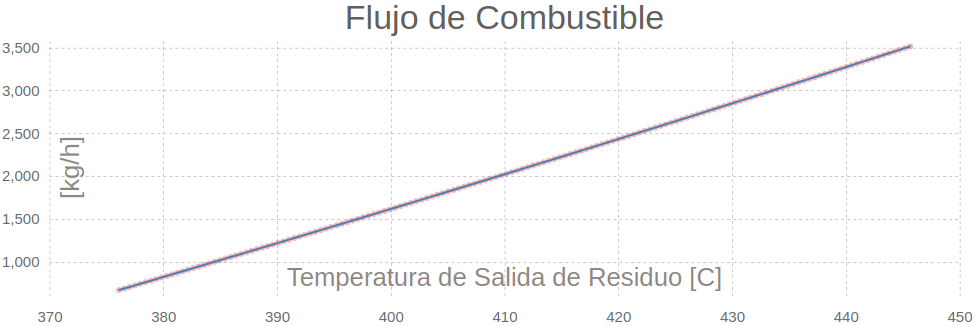
\includegraphics[scale=0.38]{images/graph-t_out-fuel}
\caption[Flujo de combustible vs Temperatura de salida de residuo]{Flujo de combustible en función de la temperatura de salida de residuo.}
\label{fig:graph-t_out-fuel}
\end{center}
\end{figure}

\par En la Figura \ref{fig:graph-t_out-fuel} se observa la necesidad de incrementar el flujo de combustible para mantener las condiciones de operación si se aumenta la temperatura a la que se desea obtener el residuo al salir del horno, este comportamiento también se observa al aumentar las otras tres posibles variables de entrada de forma independiente. Esto a consecuencia de que el combustible es la fuente de calor del horno y cualquier necesidad de energía adicional en el proceso requiere mayor flujo de combustible.

\par Al aumentar el flujo de combustible por el requerimiento de de una temperatura de salida del fluido mayor, y dejando el resto de las variables de entrada, como exceso de aire y humedad relativa, se nota un aumento en la temperatura de arco radiante (Fig. \ref{fig:graph-t_out-arc}) y por transitividad en la temperatura de salida de los gases de chimenea (Fig. \ref{fig:graph-t_out-chim}).

\begin{figure}[hbt]
\begin{center}
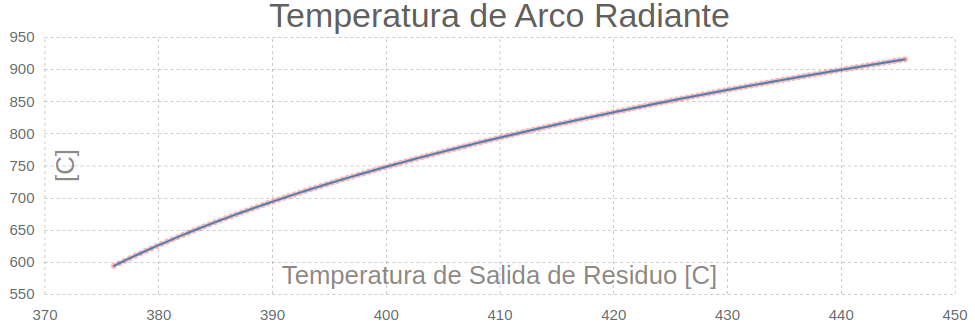
\includegraphics[scale=0.38]{images/graph-t_out-arc}
\caption[Temperatura de arco radiante vs Temperatura de salida de residuo]{Temperatura de arco radiante en función de la temperatura de salida de residuo.}
\label{fig:graph-t_out-arc}
\end{center}
\end{figure}

\begin{figure}[hbt]
\begin{center}
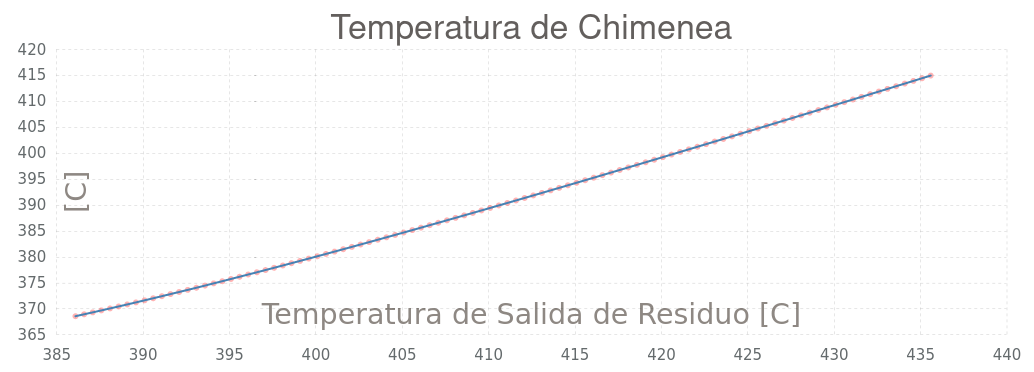
\includegraphics[scale=0.38]{images/graph-t_out-chim}
\caption[Temperatura de chimenea vs Temperatura de salida de residuo]{Temperatura de chimenea en función de la temperatura de salida de residuo.}
\label{fig:graph-t_out-chim}
\end{center}
\end{figure}

\par Para la variable de flujo de residuo también se observa la misma tendencia, siendo solo diferente la tendencia de la temperatura de arco radiante (ver la Figura \ref{fig:graph-air_excess-arc}) para el aumento exceso de aire o humedad relativa, debido que para estos dos casos la ecuación de temperatura de arco debe considerar el calor extra que se debe ceder a estos componentes en la cámara de combustión, como fue descrito en la sección de combustión de hidrocarburos.

\begin{figure}[hbt]
\begin{center}
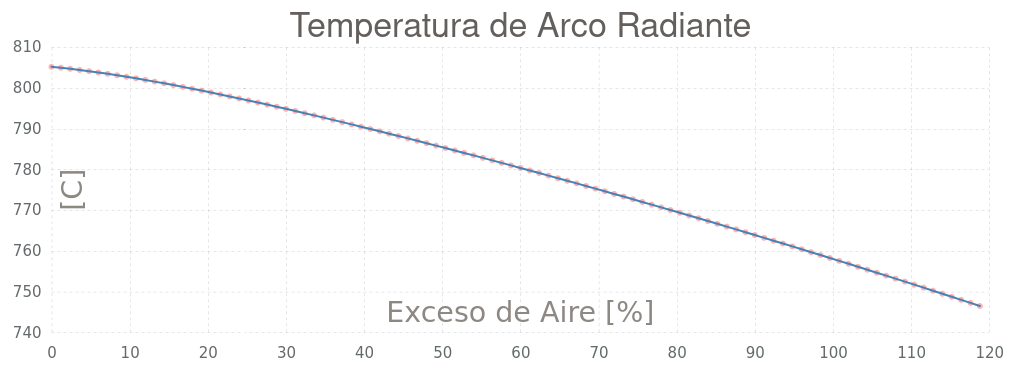
\includegraphics[scale=0.38]{images/graph-air_excess-arc}
\caption[Temperatura de arco radiante vs Exceso de aire]{Temperatura de arco radiante en función del exceso de aire en el combustible.}
\label{fig:graph-air_excess-arc}
\end{center}
\end{figure}

\par Para la variable de tasa de distribución de calor absorbido por zonas la tendencia observada en la Figura \ref{fig:graph-t_out-dist} es decreciente, lo que se traduce en que la absorción de calor disminuye en la zona radiante y aumenta en la zona convectiva. Esto debido a que la zona convectiva es más sensible al cambio de temperatura de los gases de combustión, tiene un coeficiente de transferencia de calor global mayor y un área de contacto casi diez veces mayor por la presencia de aletas. No obstante, la limitación física del material de la aletas a la temperatura no es considerada en esta simulación, para más detalle se reporta la temperatura de la punta de las aletas en la sección de resultados ampliados.

\begin{figure}[hbt]
\begin{center}
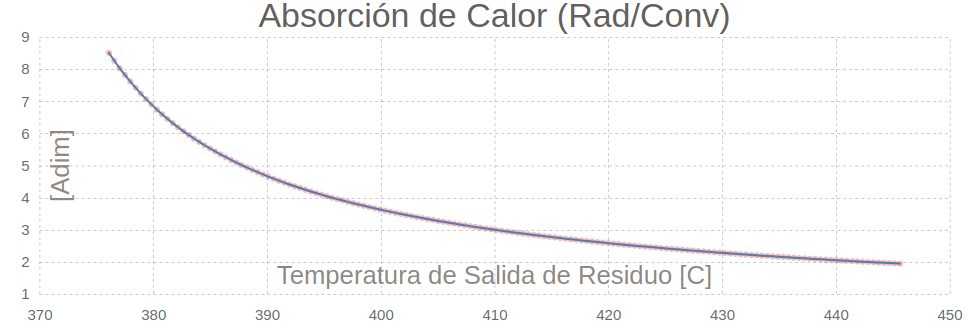
\includegraphics[scale=0.38]{images/graph-t_out-dist}
\caption[Distribución de absorción de calor vs Temperatura de salida de residuo]{Tasa de distribución de absorción de calor entre zona radiante y convectiva en función de la temperatura de salida de residuo.}
\label{fig:graph-t_out-dist}
\end{center}
\end{figure}

\par Comprobando el comportamiento esperado de la eficiencia, se observa una tendencia decreciente en la Figura \ref{fig:graph-t_out-efic}, al aumentar cualquiera de las variables de entrada seleccionadas para este análisis, un comportamiento inversamente proporcional al aumento de la temperatura de los gases en la chimenea.

\begin{figure}[hbt]
\begin{center}
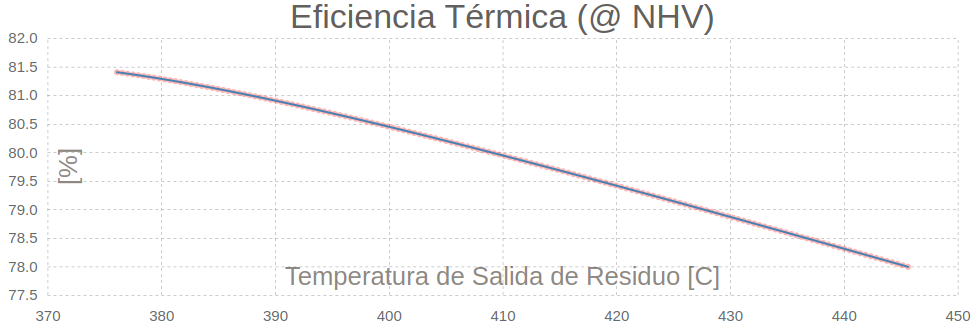
\includegraphics[scale=0.38]{images/graph-t_out-efic}
\caption[Eficiencia Térmica vs Temperatura de salida de residuo]{Eficiencia Térmica (@ Valor Calorífico Neto) en función de la temperatura de salida de residuo.}
\label{fig:graph-t_out-efic}
\end{center}
\end{figure}

\par La tendencia al incremento del flujo de combustible que se observa para todas las variables estudiadas, es directamente proporcional a las emisiones de \ac{co2}, lo que puede corroborarse en la Figura \ref{fig:graph-t_out-emi}. Este comportamiento solo varia si se usa un combustible que no genere \ac{co2}, como al elegir \ac{h2} sin ningún hidrocarburo en la mezcla, donde no existirían estas emisiones.

\begin{figure}[hbt]
\begin{center}
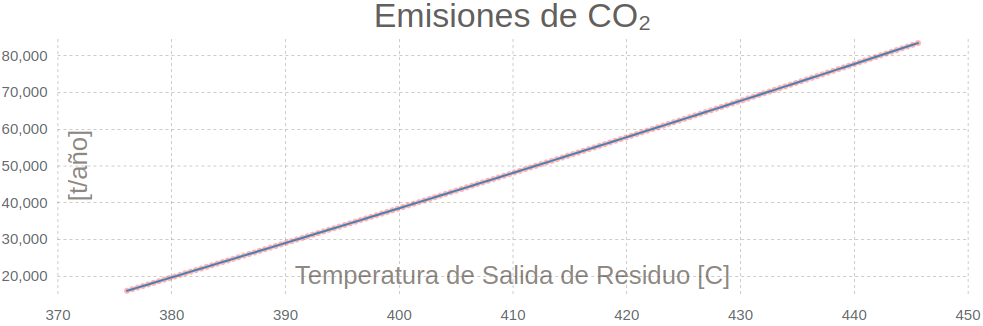
\includegraphics[scale=0.38]{images/graph-t_out-emi}
\caption[Emisiones de CO$_2$ vs Temperatura de salida de residuo]{Emisiones de CO$_2$ en función de la temperatura de salida de residuo.}
\label{fig:graph-t_out-emi}
\end{center}
\end{figure}

\section{Interfaz de usuario (UI)}

\par Sin la interfaz de usuario, el algoritmo, aunque poderoso, tendría un uso muy limitado por la complejidad que implica correrlo directamente como un programa y por lo difícil que es observar los cambios sin una amigable visualización de datos.

\par La interfaz desarrollada consiste en un sitio web donde el usuario puede navegar a distintas vistas con diferentes propósitos. A continuación se describirán dichas vistas y sus aplicaciones pensadas, esencialmente las posibilidades educativas que ofrece la comparación de dos estados del proceso, pero no limitadas a estas.

\subsection{Alcances}

\par La primera vista, que se puede apreciar en la Figura \ref{fig:alcance}, es la bienvenida a los usuarios del simulador, es una página que muestra los alcances, usos y limitaciones del simulador, la primera sección introduce el algoritmo del simulador, seguido por una descripción del horno de referencia y sus condiciones de operación.

\begin{figure}[hbt]
\begin{center}
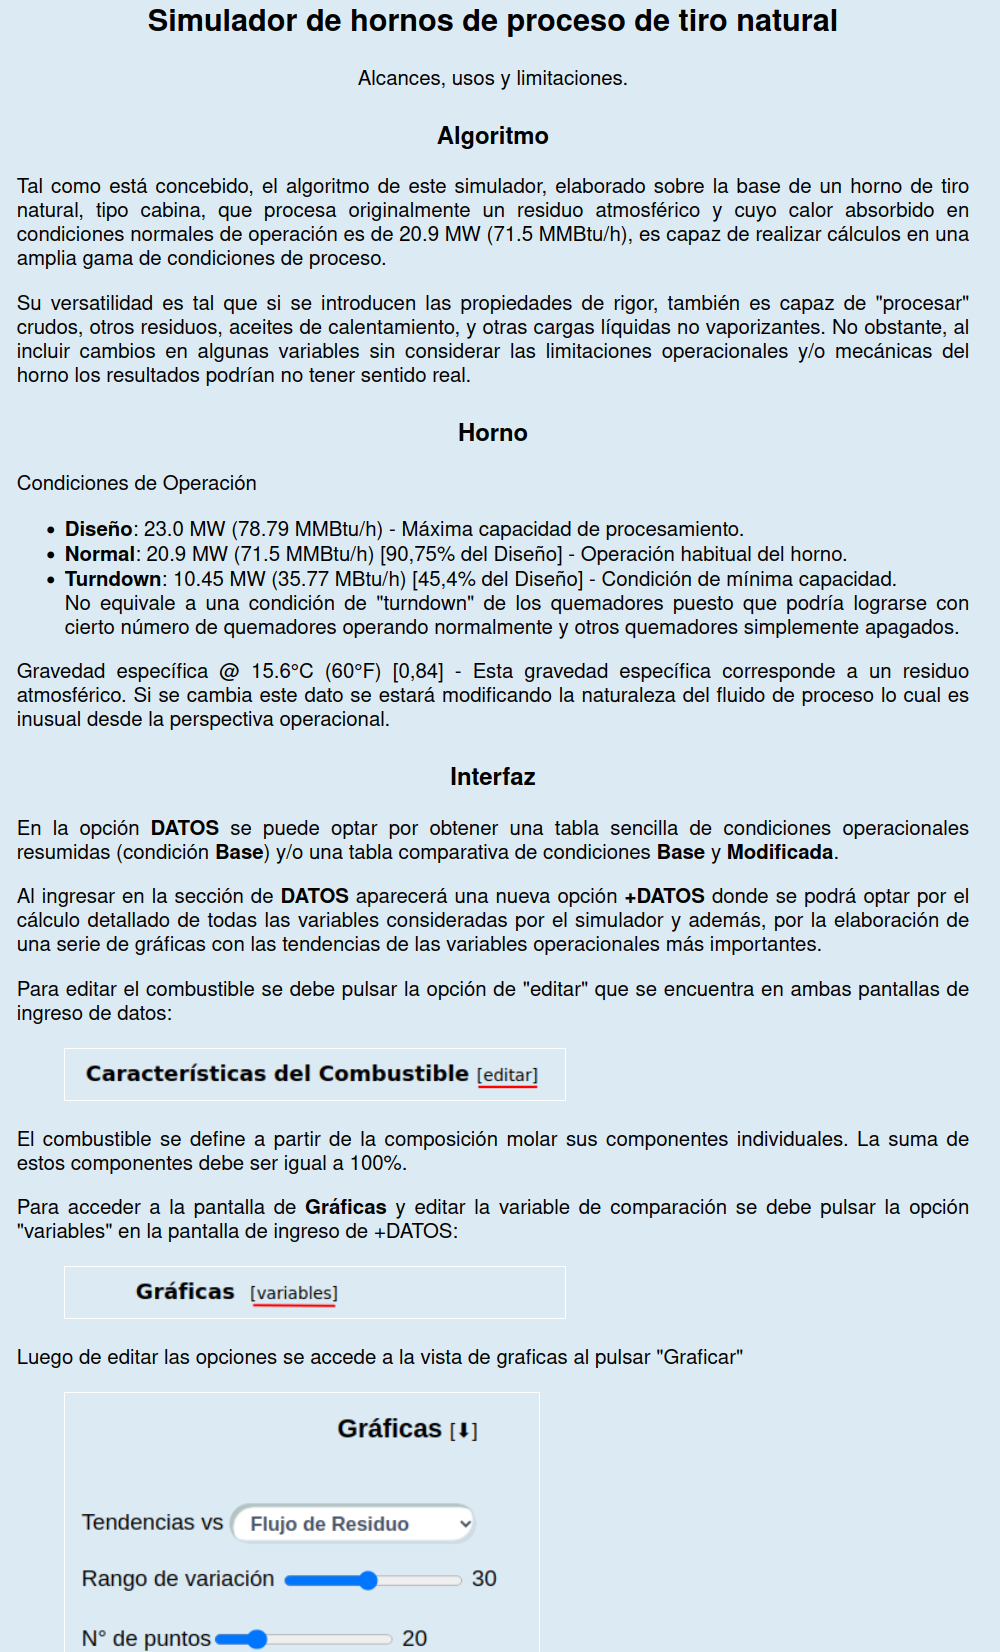
\includegraphics[scale=0.2]{images/alcance}
\caption[Página de alcances]{Página de alcances, vista introductoria a la aplicación web.}
\label{fig:alcance}
\end{center}
\end{figure}

\par La sección de interfaz describe como utilizar la barra de navegación del sitio web (ver Figura \ref{fig:navbar}), como editar el combustible a utilizar en las diferentes vistas de ingreso de datos y finalmente como usar la sección de gráficas o tendencias.

\begin{figure}[hbt]
\begin{center}

\includegraphics[scale=0.2]{images/navbar}
\caption[Barra de navegación]{Barra de navegación de la interfaz web.}
\label{fig:navbar}
\end{center}
\end{figure}

\subsection{Ingreso de datos}

\par Para la modificación de los datos de datos de entrada al simulador existen dos vistas, una resumida (ver Figura \ref{fig:datos}) que al accionar el cálculo dirige a la vista de resultados comparativos y otra vista ampliada (ver Figura \ref{fig:fulldatos}) que permite la edición de datos mas específicos y en esta vista se encuentra la posibilidad de accionar el calculo para ofrecer una página de resultados extendidos, o de graficar las tendencias escogiendo una variable a ser modificada.

\begin{figure}[hbt]
\begin{center}
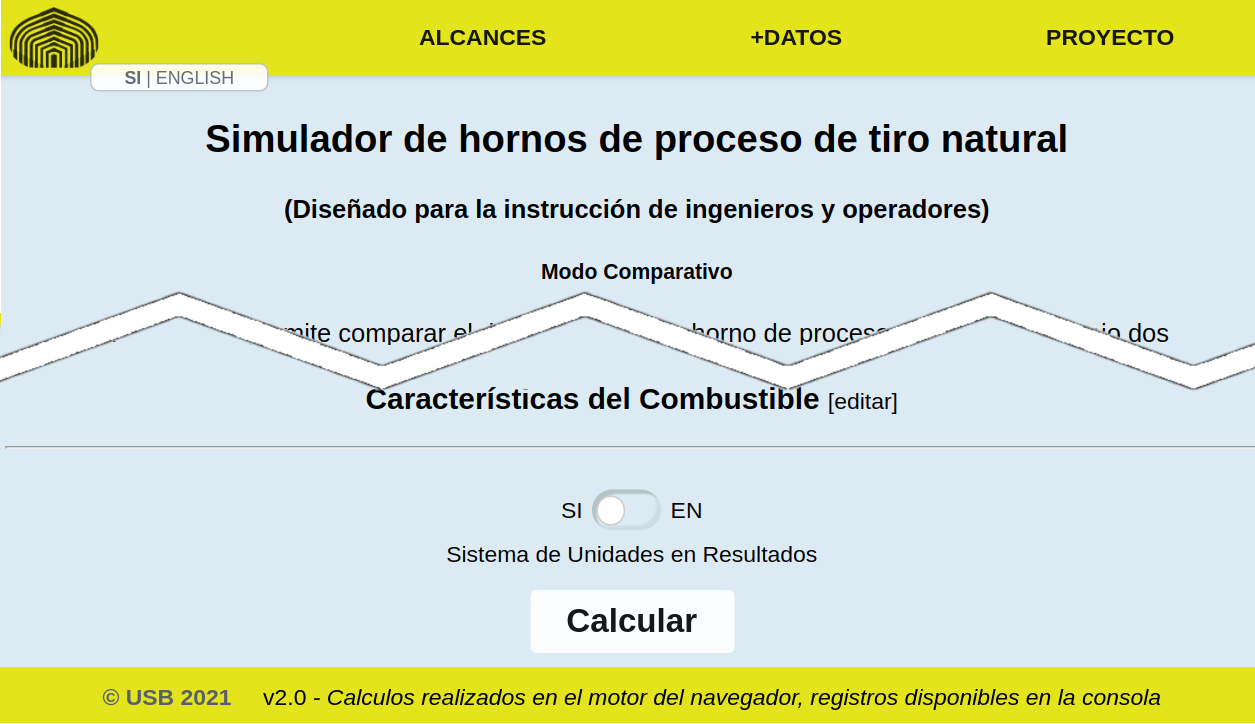
\includegraphics[scale=0.2]{images/datos}
\caption[Página de ingreso de datos para comparación]{Página de ingreso de datos utilizada para accionar el cálculo en la vista comparativa de resultados.}
\label{fig:datos}
\end{center}
\end{figure}

\begin{figure}[hbt]
\begin{center}
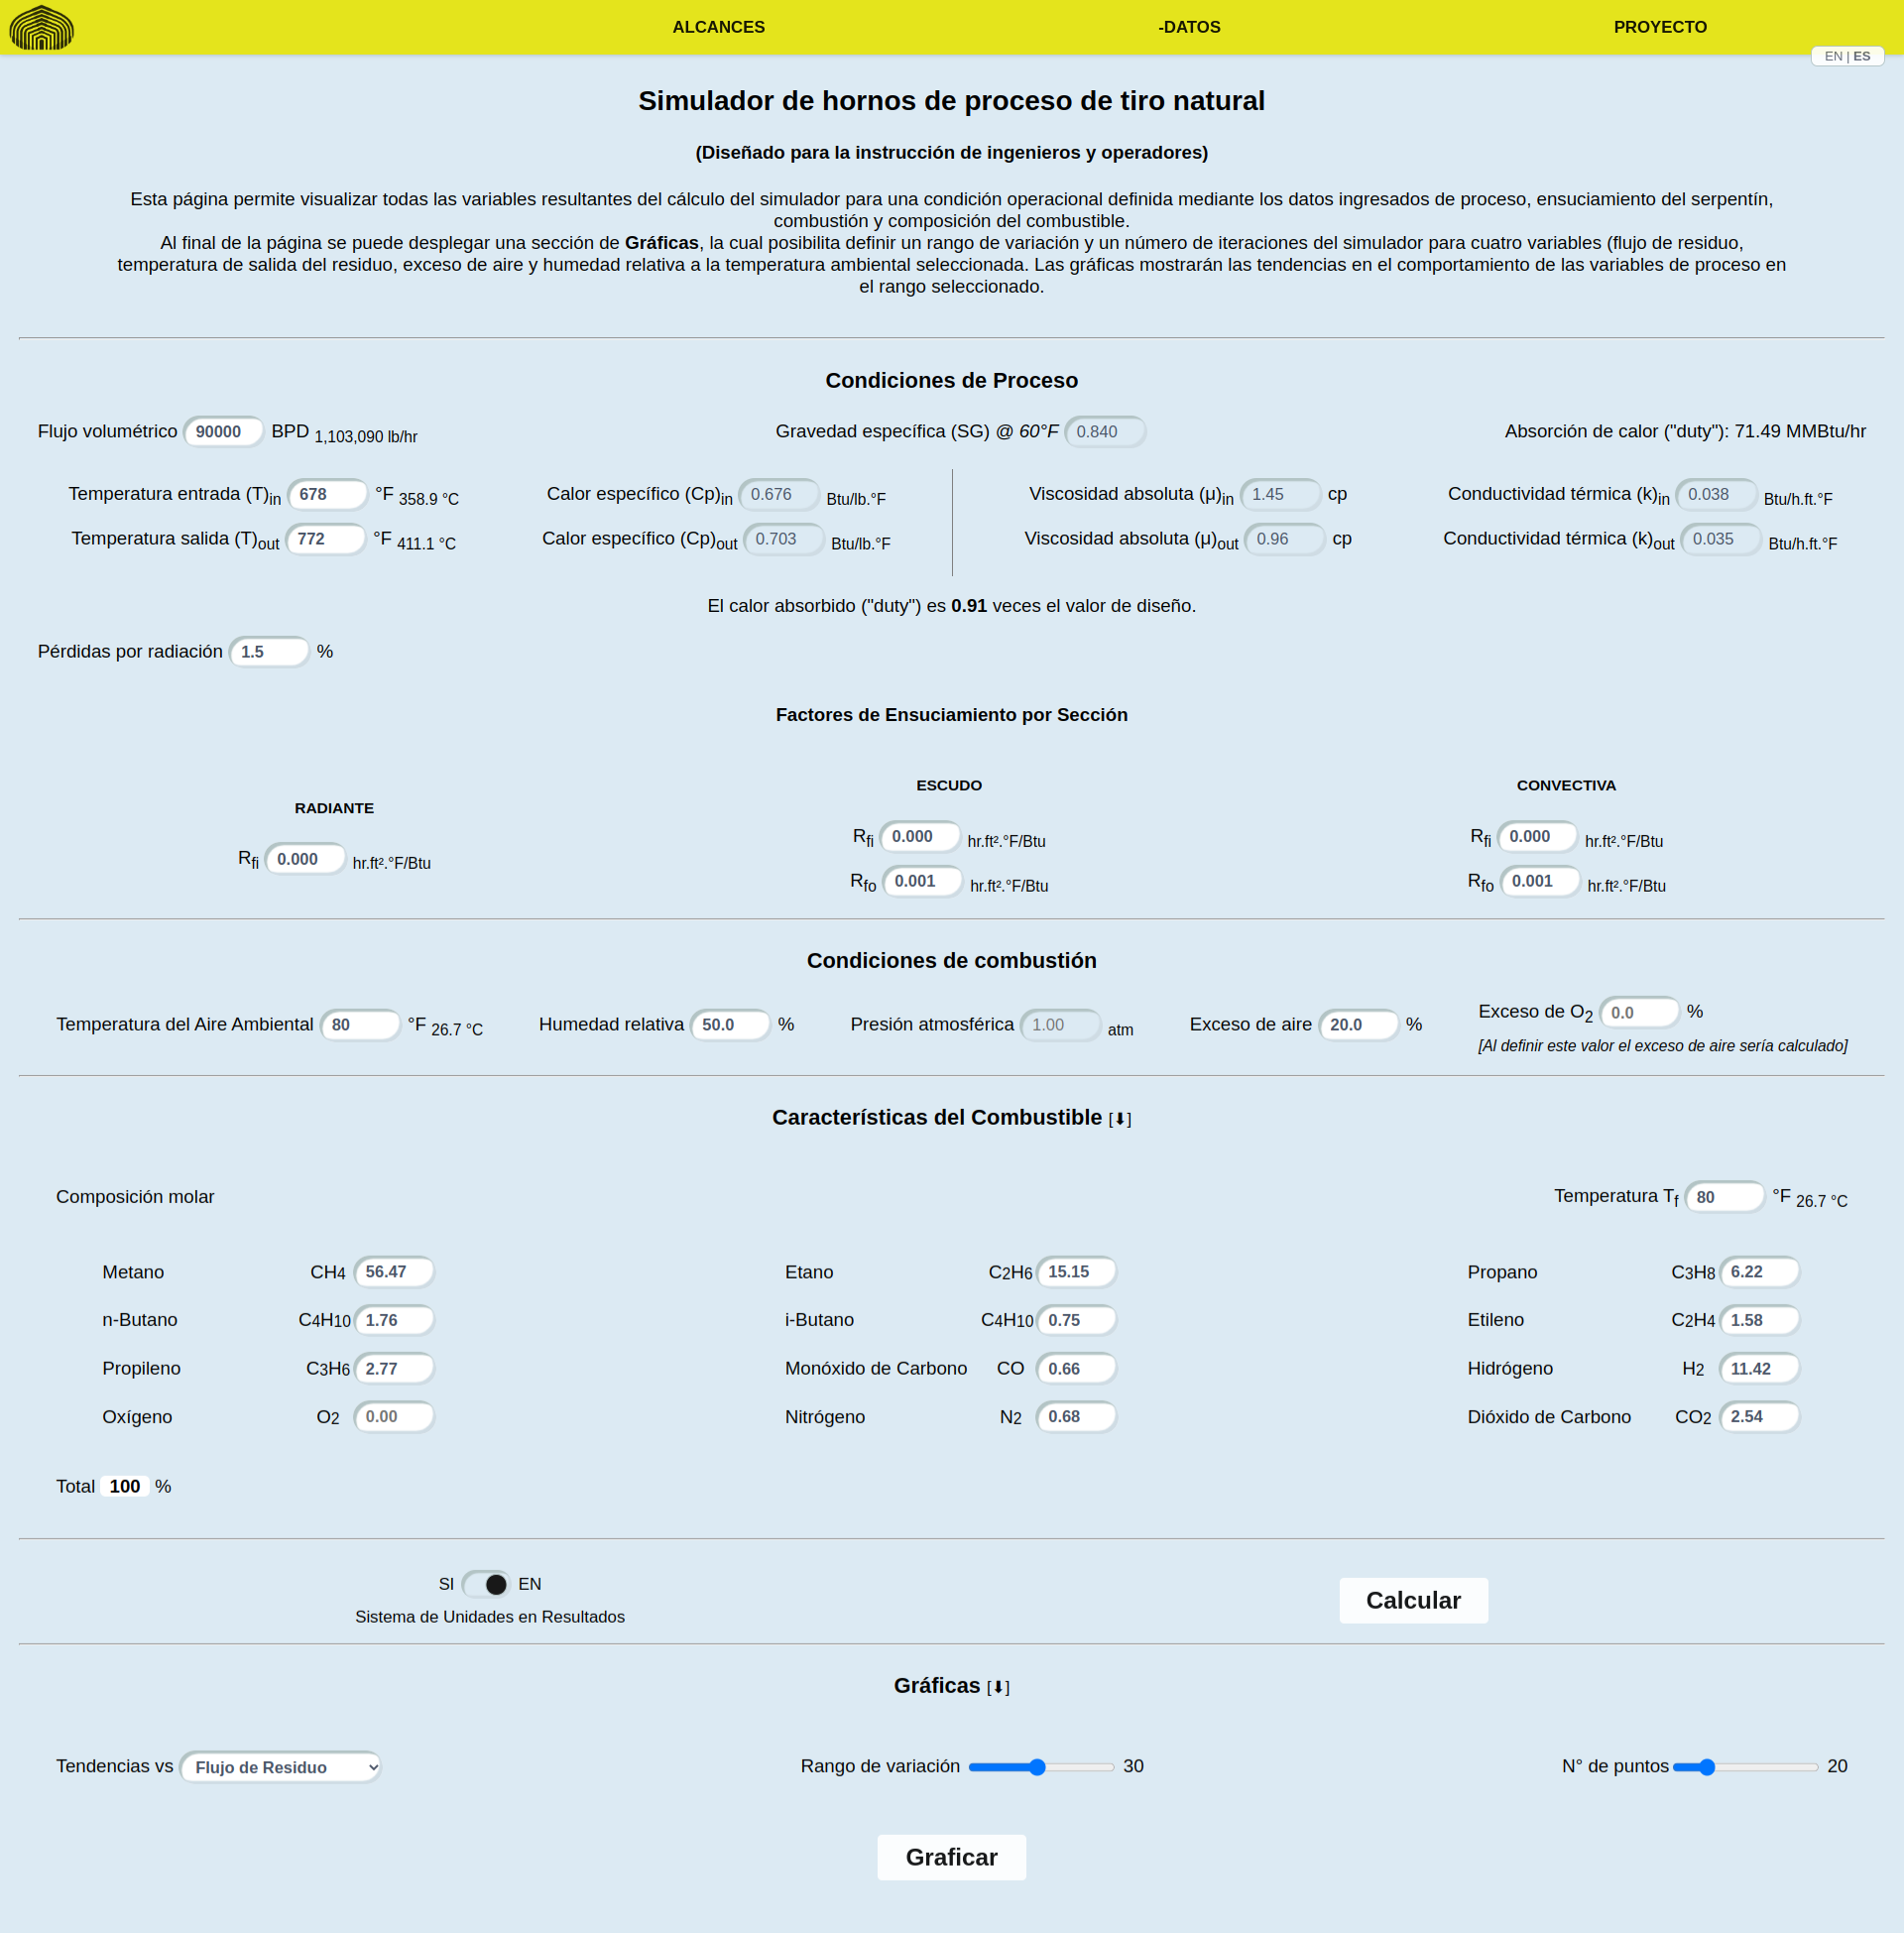
\includegraphics[scale=0.2]{images/fulldatos}
\caption[Página de ingreso de datos extendida]{Página de ingreso de datos extendida, con la opción de accionar la vista de resultados extendidos o la generación de gráficas de tendencia.}
\label{fig:fulldatos}
\end{center}
\end{figure}

\subsection{Resultados}

\par Como se describió en la sección anterior, hay dos posibles vistas para los resultados, la comparativa, de dos resultados, y la extendida de un resultado puntual. 
\subsubsection{Resultados comparativos}

\par Como se observa en la Figura \ref{fig:resultados}, es una página enfocada en comparar dos estados del horno y permitir el análisis de la consecuencia de modificar una variable desde un estado base hacia un estado modificado, siendo esto lo mas común para un operador en la industria, la recomendación es modificar solo una variable a la vez para su correcta interpretación.
\begin{figure}[hbt]
\begin{center}
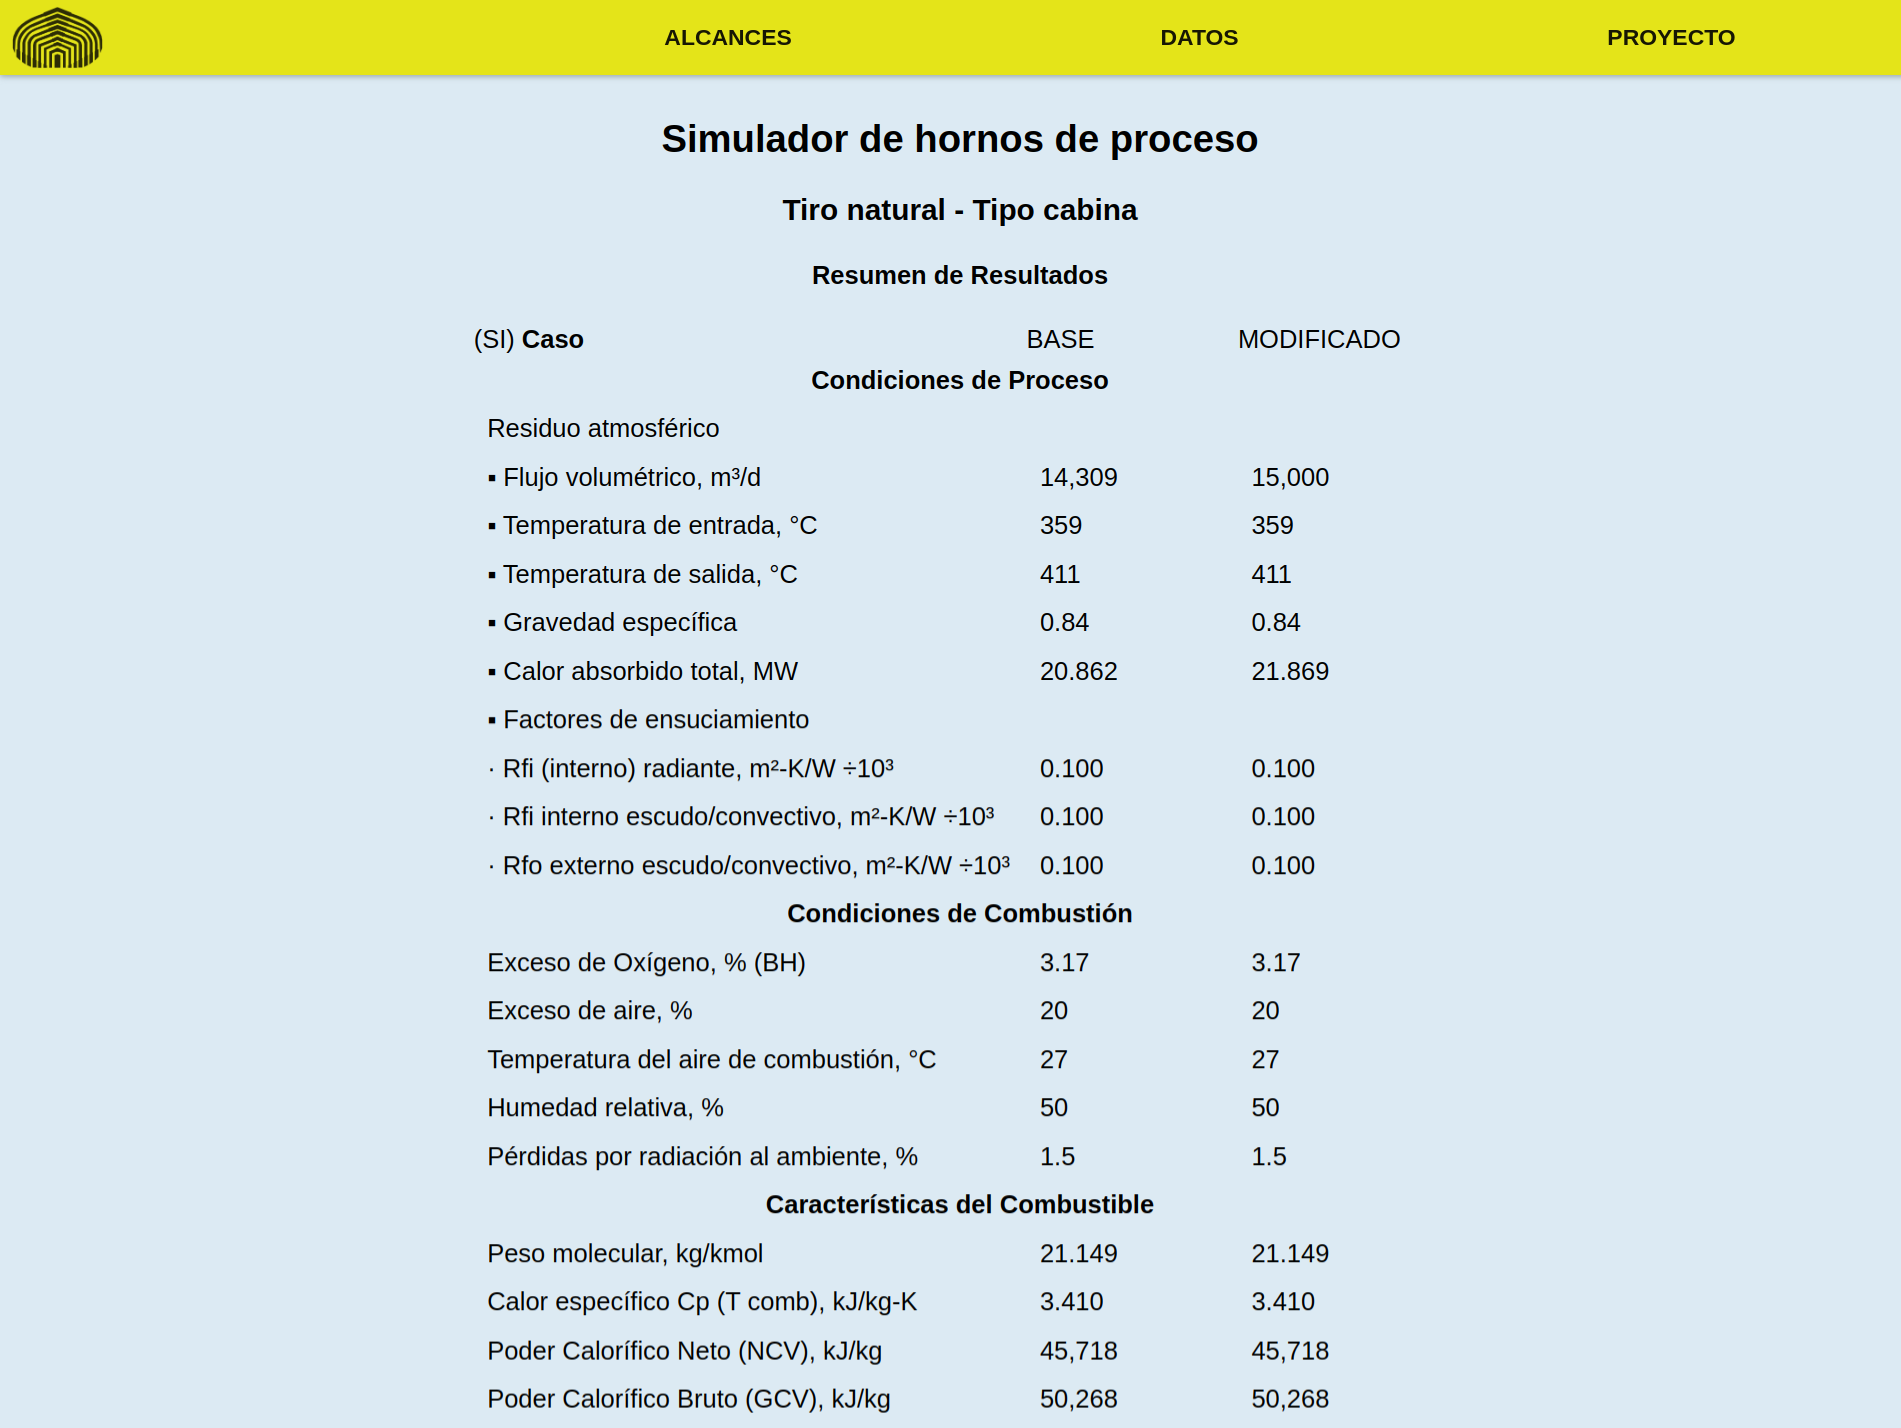
\includegraphics[scale=0.15]{images/resultadosdoble}
\caption[Página comparativa de resultados]{Página comparativa de resultados, donde se pueden detallar los cambios de un estado a otro en la operación del horno.}
\label{fig:resultados}
\end{center}
\end{figure}

\subsubsection{Resultados extendidos}
\par En esta vista (Figura \ref{fig:fullresultados}) se pueden detallar los valores obtenidos de todas las variables internas de cada sección en el simulador, su uso inicial fue al depurar las ecuaciones internas del algoritmo para encontrar sus puntos críticos y corregirlos, ahora permite apreciar las variables desglosados y seguir el comportamiento de los fenómenos desarrollados internamente.

\begin{figure}[hbt]
\begin{center}
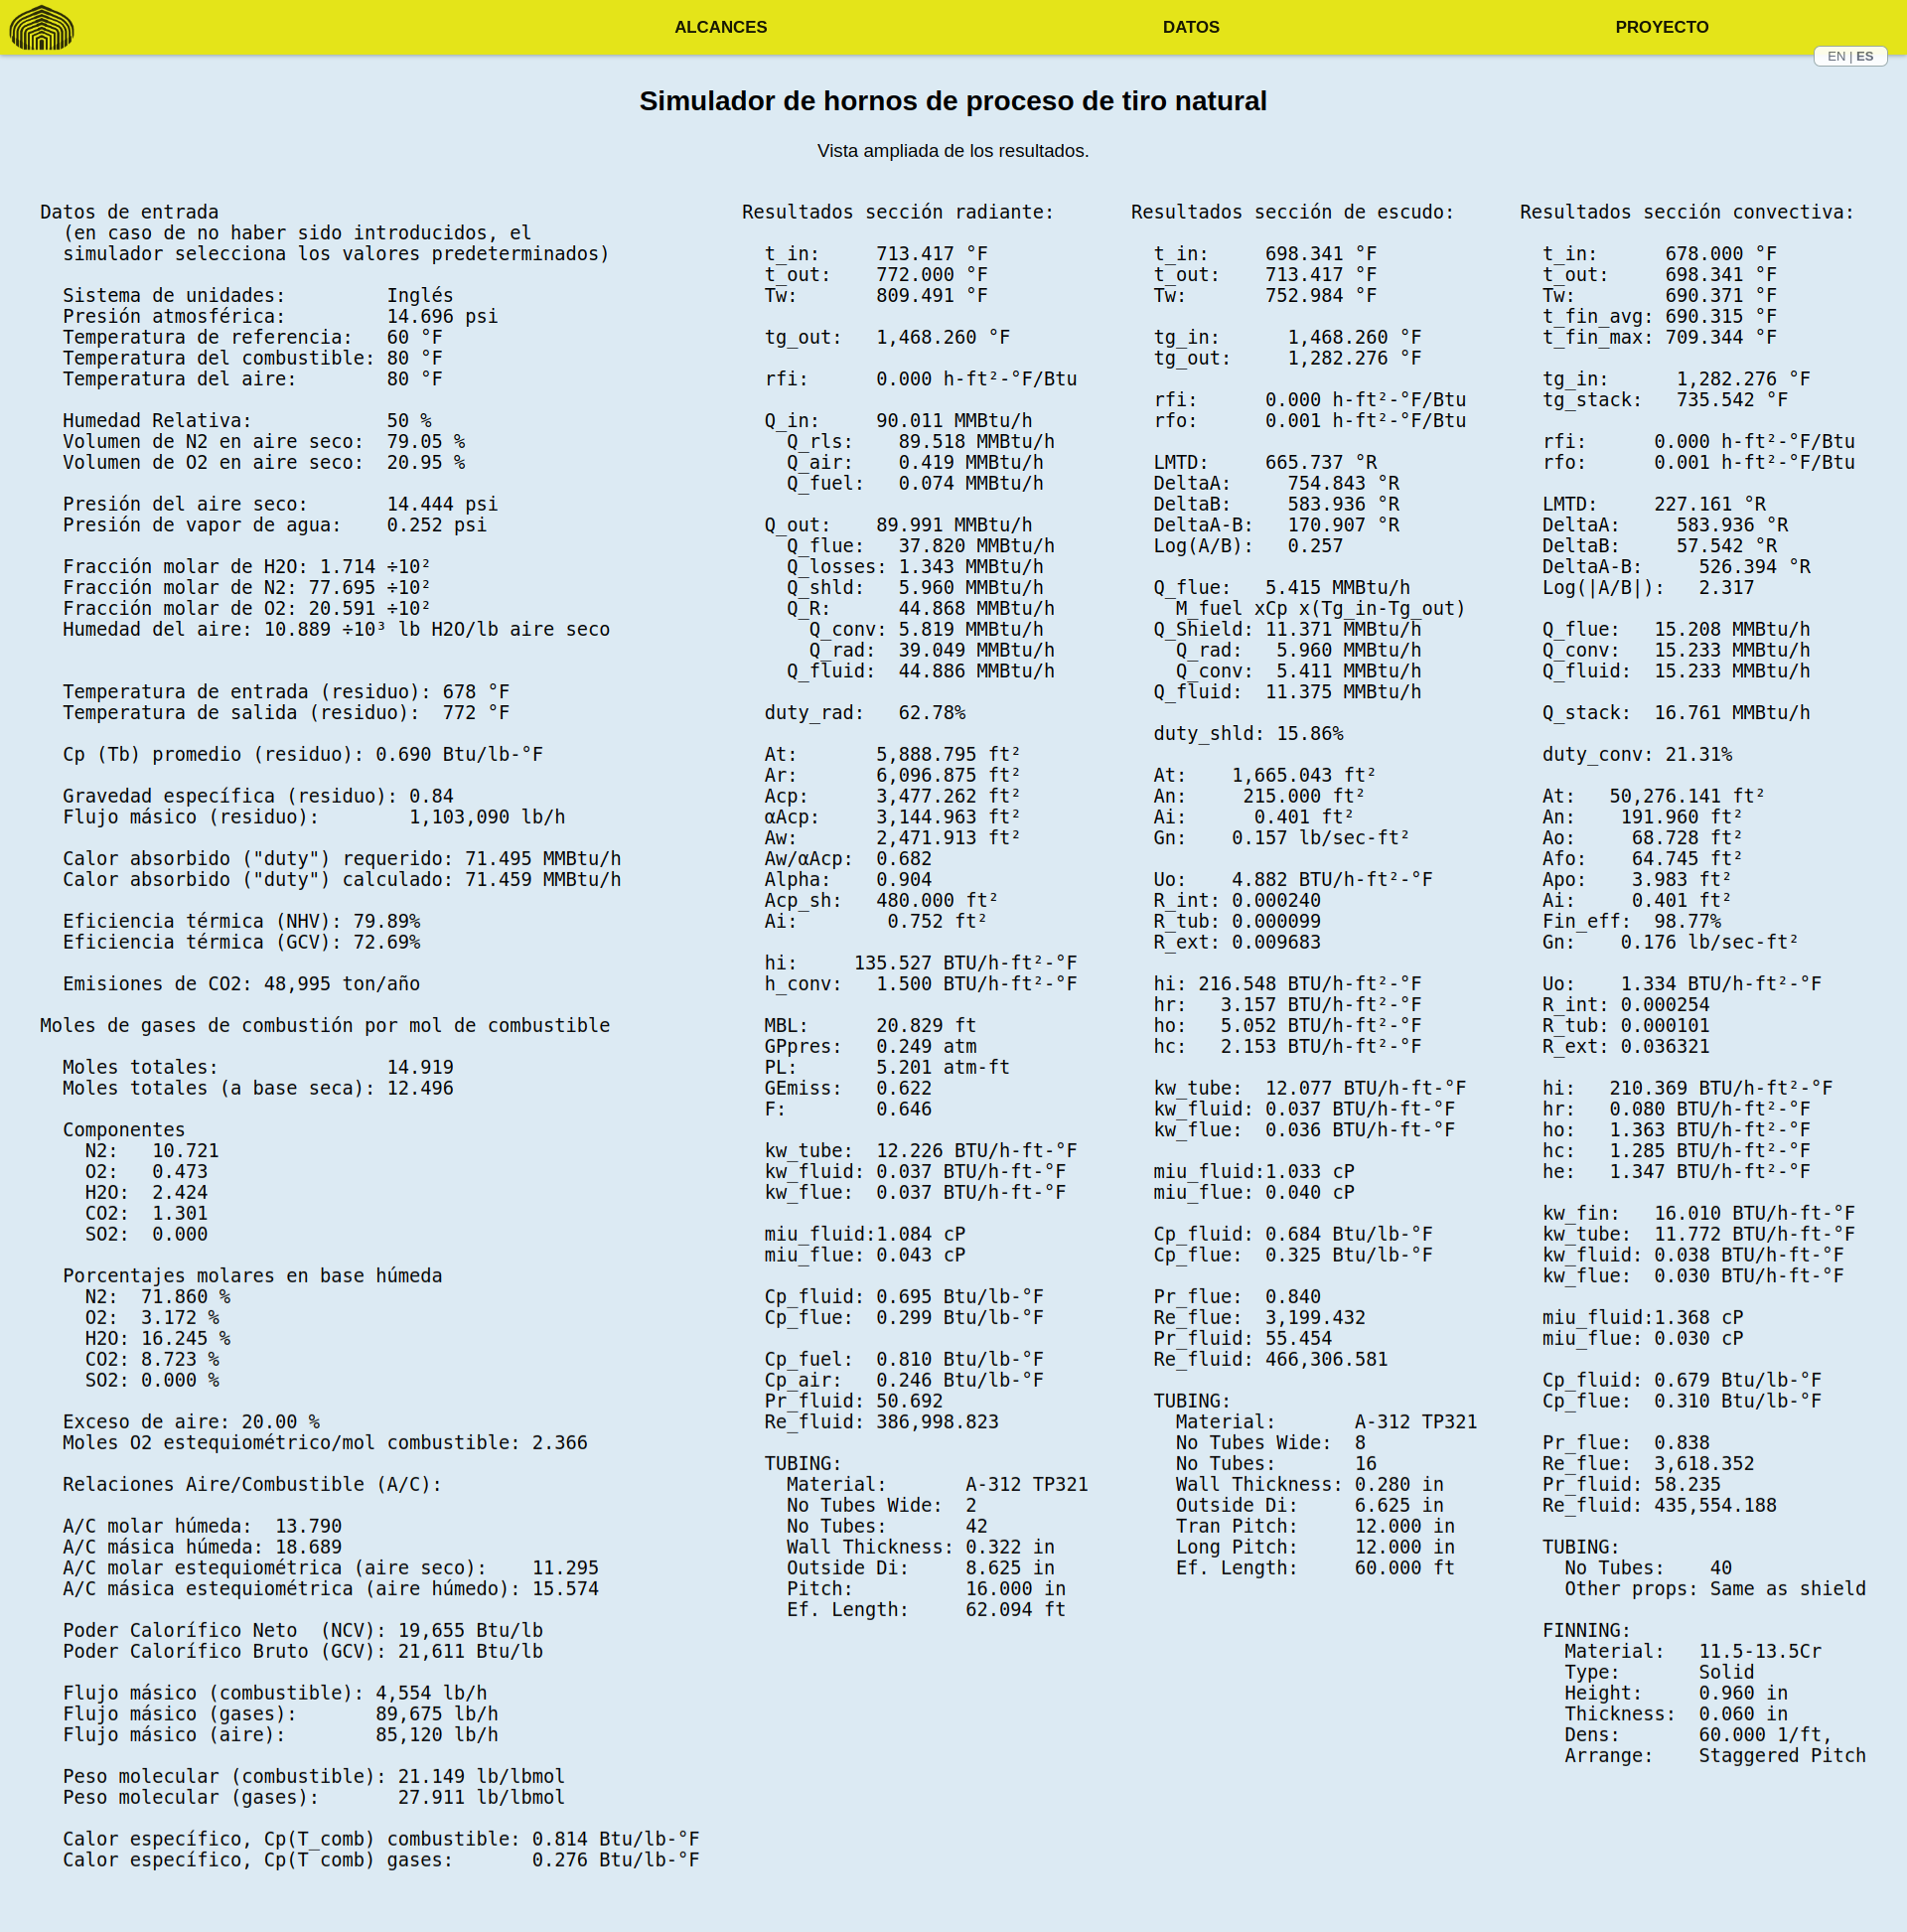
\includegraphics[scale=0.18]{images/fullresultados.png}
\caption[Página extendida de resultados]{Página extendida de resultados, donde se pueden observar a detalle las variables internas del proceso simulado.}
\label{fig:fullresultados}
\end{center}
\end{figure}

\subsection{Gráficas}

\par Esta página es pensada para los usuarios más curiosos, y para futuras modificaciones del algoritmo o extensión de sus rangos (ver Figura \ref{fig:graficas}).

\par Aquí pueden ser comprobadas las tendencias, la continuidad y la estabilidad de las variables resultantes. Fue ampliamente utilizada en el desarrollo del algoritmo para definir los detalles de los métodos numéricos usados en cada sección del simulador.

\begin{figure}[hbt]
\begin{center}
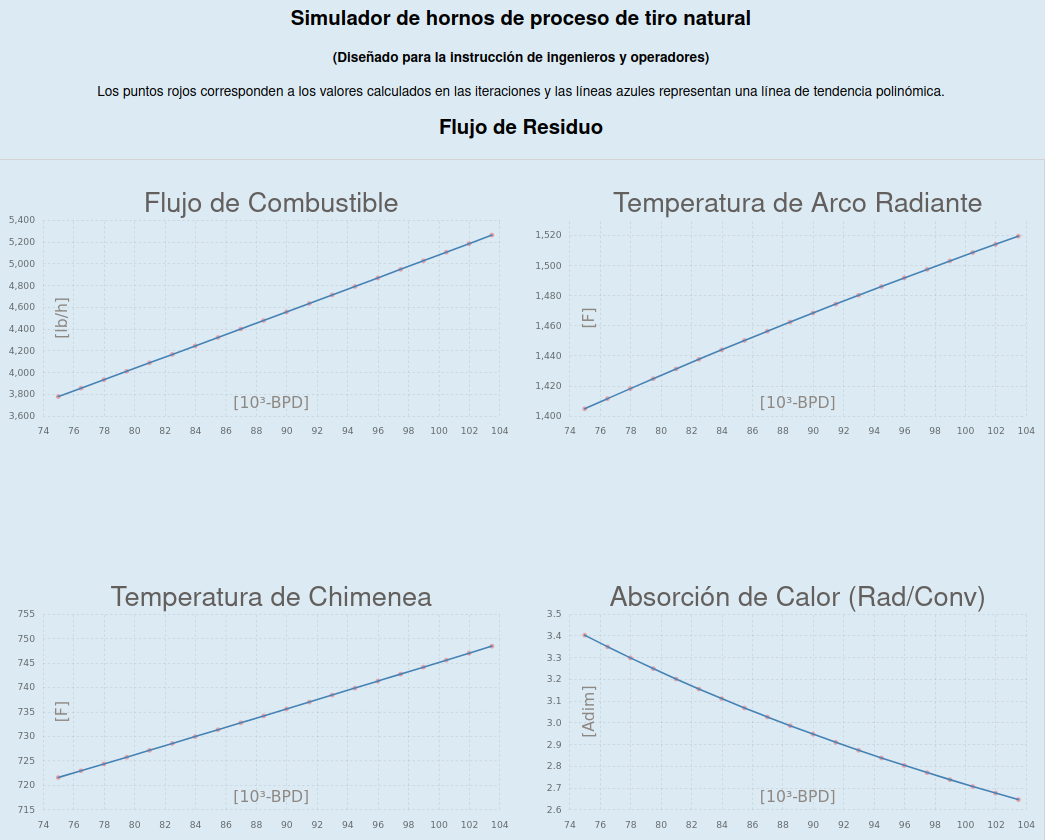
\includegraphics[scale=0.18]{images/graficas.png}
\caption[Página de gráficas]{Página de gráficas, muestra las tendencias de las variables resultantes escogidas en el rango de variación determinado por el usuario.}
\label{fig:graficas}
\end{center}
\end{figure}

% 3-      El modelo debe ser presentado como una herramienta amplia que está limitado por las características físicas del horno: área de transferencia de calor en las tres zonas de intercambio, capacidad de los quemadores y las dimensiones de la chimenea. Es decir, el diseño mecánico del horno es invariable.

% 5-      El modelo permite variar el volumen del fluido del proceso, temperatura de entrada y salida del fluido del proceso, condiciones ambientales, composición del gas de combustión y relación A/C. Las propiedades del fluido, Cp, viscosidad y gravedad específica que utiliza el modelo corresponden a la temperatura de entrada y salida y deben ser introducidas como datos. Las propiedades del gas de combustión son calculadas a partir de sus componentes.

% 6-      No existe impedimento para variar el fluido del proceso en un amplio margen de crudos con diferentes API u otras corrientes de refinería. Esto debe ser recalcado entre los puntos importantes de las virtudes del modelo.

% 7-      En forma ilustrativa, se debe mantener el fluido del diseño para demostrar la validez del modelo y  la tendencia de los resultados ante la variación de los parámetros independientes.

% 8-      Deben quedar claro las limitantes del modelo en aquellos elementos no considerados cuantitativamente (ej. formación de CO, despegue de la llama por exceso de aire, etc) y que han sido tratados mediante rangos empíricos.